\documentclass[11pt,a4paper]{article}
\usepackage[T1]{fontenc}
\usepackage{lmodern}
\usepackage[utf8]{inputenc}
\usepackage[brazil]{babel}
\usepackage[margin=2.5cm]{geometry}
\usepackage{amsmath,amssymb}
\usepackage{booktabs}
\usepackage{graphicx}
\usepackage{caption}
\usepackage{subcaption}
\usepackage[hidelinks]{hyperref}

\title{\textbf{Redes Neurais MLP}\\[0.3em]
\large Construção de baseline e estudo de ablação em problemas de regressão e classificação}
\author{Leonardo Arazo}
\date{\today}

\begin{document}
\maketitle

\begin{abstract}
\noindent
Este trabalho constrói, para dois problemas de naturezas distintas --- regressão sobre
uma função sintética e classificação de imagens no Fashion-MNIST ---, um modelo MLP
\emph{baseline} treinado com SGD puro, e avalia o efeito de quatro componentes
adicionados isoladamente: regularização L1, regularização L2, \emph{dropout} e
\emph{momentum}. Todos os experimentos usam três sementes e reportam média e desvio.
O resultado central é que os mesmos quatro componentes, sob o mesmo motor de treino e
o mesmo protocolo, produziram conclusões opostas nos dois problemas: na regressão os
três regularizadores degradaram o desempenho de forma monotônica, com ótimo em zero;
na classificação todos apresentaram melhor valor positivo, com o \emph{dropout}
reduzindo a distância entre erro de treino e de validação de $18{,}2\times$ para
$3{,}9\times$. Argumenta-se que a diferença é explicada pela quantidade de
sobreajuste disponível para ser combatida em cada problema, e que o limite de
desempenho na classificação não é de sobreajuste, mas de representação.
\end{abstract}

\section{Introdução}

O objetivo deste trabalho é duplo. Primeiro, construir empiricamente um modelo MLP de
referência (\emph{baseline}) para um problema de regressão e um de classificação,
usando exclusivamente descida de gradiente estocástica sem otimizações. Segundo,
medir o efeito de quatro componentes acrescentados individualmente a esse baseline,
mantendo a arquitetura inalterada.

A escolha de tratar os dois problemas com o mesmo código e o mesmo protocolo é
deliberada: diferenças observadas entre eles podem então ser atribuídas ao problema, e
não ao método. Como se verá na Seção~\ref{sec:discussao}, essa decisão é o que torna o
resultado principal interpretável.

\paragraph{Nota sobre terminologia.} O enunciado denomina \emph{estudo de ablação} o
procedimento adotado. No uso corrente da literatura, ablação designa a \emph{remoção}
de componentes de um sistema completo para medir a contribuição de cada um; aqui
parte-se de uma rede mínima e os componentes são \emph{acrescentados}. Mantém-se a
nomenclatura do enunciado, registrada a distinção.

\section{Metodologia}

\subsection{Protocolo experimental}

Todas as decisões --- seleção de arquitetura, de hiperparâmetros e de valores dos
componentes --- foram tomadas no conjunto de validação. O conjunto de teste foi mantido
lacrado e utilizado uma única vez por modelo, ao final.

\paragraph{Separação das fontes de aleatoriedade.} Existem duas fontes independentes de
variação: a geração do conjunto de dados e o processo de treino (inicialização de pesos
e ordem dos \emph{mini-batches}). Variá-las simultaneamente impediria atribuir qualquer
diferença observada a uma causa específica. Adotou-se, portanto, semente fixa e única
para os dados (\texttt{SEED\_DADOS = 0}) e três sementes distintas apenas para o treino
(\texttt{[1,2,3]}). Todos os modelos de um mesmo problema observam exatamente os mesmos
dados, e partem dos mesmos pesos iniciais, de modo que a diferença entre eles é o
componente adicionado.

\paragraph{Reporte estatístico.} Todos os resultados são apresentados como média $\pm$
desvio-padrão sobre as três sementes. Adota-se como critério de significância que a
diferença entre dois modelos deve exceder aproximadamente dois erros-padrão da média
para ser considerada sinal; diferenças menores são reportadas como não conclusivas.

\paragraph{Orçamento fixo de épocas.} O enunciado determina que o baseline não utilize
regularização. Como a parada antecipada (\emph{early stopping}) é uma forma de
regularização, empregá-la contaminaria o baseline com um mecanismo que deveria estar
reservado às variantes. Adotou-se, portanto, orçamento fixo de épocas, idêntico para
todos os modelos de um mesmo problema, reportando-se o estado ao final do orçamento.
O valor do orçamento foi calibrado experimentalmente antes da busca, conforme descrito
nas Seções~\ref{sec:reg-busca} e~\ref{sec:clf-orcamento}.

\subsection{Implementação}

O motor de treino foi implementado uma única vez e reutilizado integralmente nos dois
problemas. As funções de construção da rede, de treino e de fixação de sementes são
idênticas; a transição de regressão para classificação exige apenas três alterações:
a dimensionalidade de entrada e saída ($1\to1$ contra $784\to10$), a função de custo
(erro quadrático médio contra entropia cruzada) e a função de métricas.

Duas decisões de implementação merecem registro. A camada de saída não possui função
de ativação em nenhum dos dois casos: na regressão porque o alvo é um número real
arbitrário; na classificação porque \texttt{nn.CrossEntropyLoss} aplica
\emph{log-softmax} internamente, e uma aplicação adicional degradaria o treino
silenciosamente. Além disso, a regularização L2 é obtida pelo parâmetro
\texttt{weight\_decay} do otimizador --- a derivada de
$\frac{\lambda}{2n}\sum_w w^2$ é $\frac{\lambda}{n}w$, exatamente o termo somado ao
gradiente ---, ao passo que a L1 exige implementação manual, por $|w|$ não possuir
derivada analítica embutida. Na L1 excluíram-se os termos de viés da penalização.
Registra-se a assimetria resultante: o \texttt{weight\_decay} do PyTorch penaliza
também os vieses.

\section{Problema 1: Regressão}

\subsection{Geração dos dados}

O enunciado determina a geração de uma função não trivial de uma variável
independente, contendo não linearidades, descontinuidades e ruído. Adotou-se

\begin{equation}
f(x) = \sin(3x) + 0{,}3x + 1{,}5\cdot\mathbf{1}[x>2] + \varepsilon,
\qquad x \sim \mathcal{U}(-5,5), \quad \varepsilon \sim \mathcal{N}(0,\,0{,}2^2),
\end{equation}

com $n=300$ pontos, divididos em 210 para treino, 45 para validação e 45 para teste.
Cada termo cumpre uma função distinta: o termo linear é trivialmente aprendido e serve
de verificação de sanidade; o termo senoidal, com aproximadamente 4{,}8 períodos no
domínio, é o que discrimina arquiteturas; e a descontinuidade em $x=2$ constitui um
limite representacional, discutido na Seção~\ref{sec:degrau}.

A amostragem de $x$ é uniforme e aleatória, e não em grade regular, de modo que as
lacunas irregulares entre pontos permitam observar o comportamento interpolatório da
rede. As variáveis foram padronizadas com média e desvio calculados \emph{exclusivamente}
sobre o conjunto de treino, e as métricas revertidas à escala original de $f(x)$.

\paragraph{Escolha de $n$.} O número de amostras controla diretamente a possibilidade de
sobreajuste e, portanto, a possibilidade de os regularizadores exibirem qualquer efeito.
Verificou-se $n=150$ por precaução, obtendo-se $R^2 = 0{,}9683$ contra $0{,}9704$ de
$n=300$, valores estatisticamente equivalentes; manteve-se $n=300$.

\subsection{Teto de desempenho}

Com $\operatorname{Var}(y) = 3{,}056$ e $\operatorname{Var}(\varepsilon) = 0{,}04$, o
desempenho máximo alcançável por qualquer modelo é

\begin{equation}
R^2_{\max} = 1 - \frac{0{,}04}{3{,}056} = 0{,}987,
\qquad \mathrm{MSE}_{\text{irredutível}} = 0{,}04.
\end{equation}

Todos os resultados devem ser lidos contra esse teto. Um $R^2$ próximo de $1{,}0$ não
indicaria excelência, mas ajuste ao ruído.

\subsection{Busca do baseline}
\label{sec:reg-busca}

Adotou-se busca coordenada: varre-se um eixo mantendo os demais congelados, fixa-se o
melhor valor e prossegue-se ao eixo seguinte. O procedimento produz aproximadamente dez
execuções, contra as dezenas de uma busca exaustiva, e gera tabelas interpretáveis por
eixo.

\paragraph{Calibração prévia do orçamento.} Sondagens iniciais com 3.000 épocas
indicaram que a perda de validação ainda decrescia ao final do orçamento (mínimo na
época 2.967 de 3.000), configurando treino interrompido e não sobreajuste. Nesse regime,
regularizadores só poderiam degradar o desempenho. Com 10.000 épocas, o erro de treino
atinge $0{,}0106$ --- \emph{abaixo} do piso de ruído padronizado ($0{,}0131$) ---, contra
$0{,}0197$ de validação, caracterizando sobreajuste. Adotou-se 10.000 épocas.

Registra-se um achado metodológico relevante: nas sondagens com 3.000 épocas, a
topologia \texttt{[128]} aparecia inferior a \texttt{[64]} ($0{,}9105$ contra
$0{,}9314$), ao passo que com 10.000 épocas a ordem se inverte ($0{,}9516$ contra
$0{,}8822$). Redes maiores convergem mais lentamente; \textbf{comparar arquiteturas sob
orçamento insuficiente inverte o ranking}, o que justifica calibrar o orçamento antes
da busca.

\begin{table}[htbp]
\centering
\caption{Busca coordenada para regressão. Métricas em validação, 3 sementes, 10.000 épocas.}
\label{tab:reg-busca}
\begin{tabular}{llcc}
\toprule
Eixo & Valor & $R^2$ & RMSE \\
\midrule
Largura & \texttt{[16]} & $0{,}8633 \pm 0{,}0291$ & 0{,}6290 \\
        & \texttt{[32]} & $0{,}8770 \pm 0{,}0551$ & 0{,}5824 \\
        & \texttt{[64]} & $0{,}8822 \pm 0{,}0730$ & 0{,}5610 \\
        & \texttt{[128]} & $\mathbf{0{,}9516 \pm 0{,}0051}$ & 0{,}3761 \\
\midrule
Profundidade & \texttt{[128]} & $0{,}9516 \pm 0{,}0051$ & 0{,}3761 \\
             & \texttt{[128,128]} & $0{,}9756 \pm 0{,}0022$ & 0{,}2671 \\
             & \texttt{[128,128,128]} & $\mathbf{0{,}9780 \pm 0{,}0012}$ & 0{,}2539 \\
\midrule
Taxa de aprendizado & $0{,}01$ & $0{,}9742 \pm 0{,}0031$ & 0{,}2745 \\
                    & $0{,}05$ & $\mathbf{0{,}9780 \pm 0{,}0012}$ & 0{,}2539 \\
                    & $0{,}10$ & $0{,}9763 \pm 0{,}0007$ & 0{,}2634 \\
\bottomrule
\end{tabular}
\end{table}

\paragraph{Baseline adotado: \texttt{[128,128]}, $\text{lr}=0{,}05$.} A busca maximizou
$R^2$ e apontou \texttt{[128,128,128]}. Adotou-se, contudo, a rede de duas camadas: a
terceira camada rende $+0{,}0024$ de $R^2$ ao custo de dobrar o número de parâmetros
(de 16.897 para 33.409), e $0{,}0024$ é da ordem do próprio desvio entre sementes
($0{,}0022$). Pelo critério estabelecido na metodologia, o ganho não constitui sinal.

Observa-se, adicionalmente, que o desvio entre sementes decresce à medida que o modelo
melhora ($0{,}073$ em \texttt{[64]}, $0{,}005$ em \texttt{[128]}, $0{,}001$ em
\texttt{[128,128,128]}): modelos subdimensionados dependem substancialmente mais da
inicialização.

\subsection{Estudo de ablação}

\begin{table}[htbp]
\centering
\caption{Ablações na regressão. Baseline \texttt{[128,128]}, lr $0{,}05$,
$R^2 = 0{,}9756 \pm 0{,}0022$. Validação, 3 sementes.}
\label{tab:reg-abl}
\begin{tabular}{llcr}
\toprule
Componente & Valor & $R^2$ & $\Delta R^2$ \\
\midrule
L1 & $10^{-6}$ & $0{,}9754 \pm 0{,}0028$ & $-0{,}0002$ \\
   & $10^{-5}$ & $0{,}9749 \pm 0{,}0024$ & $-0{,}0006$ \\
   & $10^{-4}$ & $0{,}9738 \pm 0{,}0015$ & $-0{,}0018$ \\
\midrule
L2 & $10^{-5}$ & $0{,}9755 \pm 0{,}0025$ & $-0{,}0000$ \\
   & $10^{-4}$ & $0{,}9744 \pm 0{,}0026$ & $-0{,}0011$ \\
   & $10^{-3}$ & $0{,}9631 \pm 0{,}0060$ & $-0{,}0125$ \\
\midrule
Dropout & $0{,}1$ & $0{,}9745 \pm 0{,}0026$ & $-0{,}0011$ \\
        & $0{,}2$ & $0{,}9689 \pm 0{,}0016$ & $-0{,}0067$ \\
        & $0{,}5$ & $0{,}9225 \pm 0{,}0031$ & $-0{,}0531$ \\
\midrule
Momentum & $0{,}5$  & $0{,}9776 \pm 0{,}0010$ & $+0{,}0021$ \\
         & $0{,}9$  & $0{,}9493 \pm 0{,}0180$ & $-0{,}0263$ \\
         & $0{,}99$ & $0{,}2175 \pm 0{,}3863$ & $-0{,}7581$ \\
\bottomrule
\end{tabular}
\end{table}

Os três regularizadores degradam o desempenho de forma \emph{monotônica}, e nos três o
melhor valor é o menor testado --- isto é, situado na borda inferior da faixa. Estender a
faixa nessa direção equivale a caminhar para $\lambda \to 0$, que é o próprio baseline.
A leitura correta é que \textbf{o valor ótimo dos três regularizadores é zero}.

O resultado possui explicação mecânica: a distância entre erro de treino e de validação
é modesta ($0{,}0106$ contra $0{,}0197$), não há degradação temporal a corrigir, e o
$R^2$ de $0{,}9756$ dista apenas $0{,}011$ do teto imposto pelo ruído. Não resta
variância suficiente para compensar o viés introduzido pela penalização.

O comportamento do momentum é previsível pela relação entre passo efetivo e coeficiente,
$\text{lr}_{\text{ef}} \approx \text{lr}/(1-\beta)$. Para $\beta = 0{,}5$ obtém-se
$\text{lr}_{\text{ef}} = 0{,}10$, valor que na Tabela~\ref{tab:reg-busca} rendeu
$0{,}9763$; para $\beta = 0{,}99$, $\text{lr}_{\text{ef}} = 5{,}0$, e o desvio
($0{,}3863$) superior à própria média indica divergência completa em ao menos uma
semente. Ressalta-se que o momentum é o único dos quatro componentes que não constitui
regularização, mas aceleração.

\subsection{Resultados no conjunto de teste}

\begin{table}[htbp]
\centering
\caption{Resultados finais da regressão. Conjunto de teste, acessado uma única vez.}
\label{tab:reg-teste}
\begin{tabular}{lccccc}
\toprule
Modelo & $R^2$ (validação) & $R^2$ (teste) & MAE & RMSE & Degradação \\
\midrule
Baseline      & $0{,}9756 \pm 0{,}0022$ & $0{,}9829 \pm 0{,}0018$ & 0{,}1922 & 0{,}2372 & 0{,}912 \\
L1 $10^{-6}$  & $0{,}9754 \pm 0{,}0028$ & $0{,}9828 \pm 0{,}0022$ & 0{,}1937 & 0{,}2378 & 0{,}901 \\
L2 $10^{-5}$  & $0{,}9755 \pm 0{,}0025$ & $0{,}9828 \pm 0{,}0023$ & 0{,}1930 & 0{,}2376 & 0{,}905 \\
Dropout $0{,}1$ & $0{,}9745 \pm 0{,}0026$ & $0{,}9783 \pm 0{,}0034$ & 0{,}2193 & 0{,}2667 & 0{,}903 \\
Momentum $0{,}5$ & $0{,}9776 \pm 0{,}0010$ & $\mathbf{0{,}9842 \pm 0{,}0020}$ & 0{,}1879 & 0{,}2277 & 0{,}915 \\
\bottomrule
\end{tabular}
\end{table}

A coluna \emph{degradação} corresponde à razão entre a média da perda de validação nas
últimas mil épocas e a média em mil épocas centrais do treino; valores superiores a
$1$ indicam piora. Todos os modelos situam-se em torno de $0{,}91$, isto é, a validação
ainda melhorava ao final do orçamento. \textbf{Não há sobreajuste temporal na
regressão}; o sobreajuste presente é estrutural, manifesto na distância entre treino e
validação.

Duas observações. Primeiro, o desempenho no teste superou o de validação em todos os
modelos ($\approx 0{,}983$ contra $\approx 0{,}976$); com apenas 45 pontos em cada
partição, a diferença é variação amostral e não deve ser interpretada como
generalização superior. Segundo, a ordenação dos modelos é idêntica nas duas partições,
o que evidencia que a seleção por validação não enviesou a conclusão final. O ganho do
momentum $0{,}5$ no teste ($+0{,}0013$) permanece dentro da variação entre sementes e
não é, portanto, demonstrável.

\subsection{Limite representacional na descontinuidade}
\label{sec:degrau}

\begin{figure}[htbp]
\centering
\begin{subfigure}{0.49\textwidth}
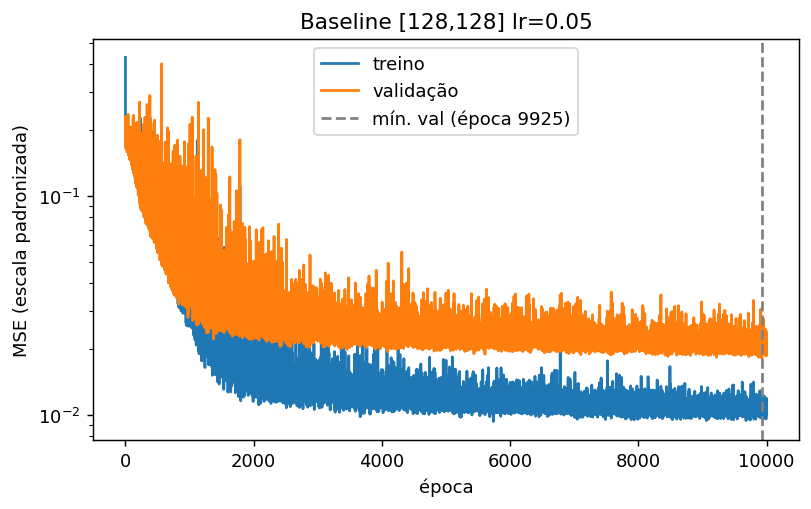
\includegraphics[width=\linewidth]{curva_baseline.png}
\caption{Evolução do treino e da validação.}
\end{subfigure}
\hfill
\begin{subfigure}{0.49\textwidth}
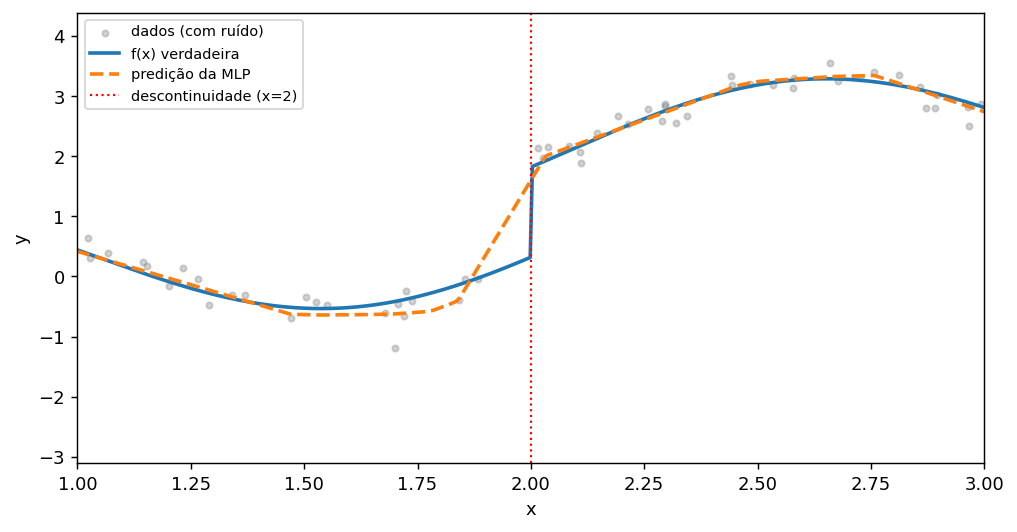
\includegraphics[width=\linewidth]{ajuste_zoom_degrau.png}
\caption{Ajuste na região da descontinuidade.}
\end{subfigure}
\caption{Baseline da regressão (\texttt{[128,128]}, lr $0{,}05$). À esquerda, escala
logarítmica; à direita, ampliação em torno de $x=2$.}
\label{fig:reg}
\end{figure}

A Figura~\ref{fig:reg}(b) evidencia o limite representacional previsto. Onde $f(x)$
apresenta salto vertical em $x=2$, a rede produz uma rampa de largura aproximada
$0{,}17$, iniciada em $x \approx 1{,}85$, antecipando a descontinuidade; observa-se
ainda leve subestimação na região $1{,}4 \le x \le 1{,}8$.

O fenômeno não decorre de treino insuficiente nem de capacidade inadequada. Uma MLP é
uma composição de funções contínuas e, portanto, \emph{não pode} representar uma
descontinuidade --- apenas aproximá-la por uma rampa de inclinação finita, linear por
partes no caso da ativação ReLU. Aumentar a capacidade estreita a rampa, mas não a
elimina.

\section{Problema 2: Classificação}

\subsection{Dados e preparação}

Utilizou-se o Fashion-MNIST: 60.000 imagens de treino e 10.000 de teste, $28\times28$
em tons de cinza, dez classes balanceadas. Preservou-se o conjunto de teste oficial e
extraíram-se 10.000 imagens do treino para validação, resultando em 50.000/10.000/10.000
--- proporções coerentes com as adotadas na regressão e comparáveis com a literatura.

A padronização utilizou média e desvio \emph{escalares} calculados sobre o treino
($\mu = 0{,}2858$, $\sigma = 0{,}3528$), e não por pixel: os pixels de borda são quase
sempre nulos e apresentariam desvio aproximadamente zero, produzindo divisões inválidas.
Adotou-se \emph{batch} de 128, contra 32 na regressão, dado que o conjunto é 238 vezes
maior; registra-se que \emph{batches} maiores produzem gradientes menos ruidosos, e que
o ruído do \emph{mini-batch} constitui em si uma regularização implícita leve.

\paragraph{Perda da estrutura espacial.} A conversão $28\times28 \to 784$ elimina a
noção de vizinhança entre pixels: a rede recebe 784 valores independentes e uma
permutação fixa das colunas produziria resultado idêntico. Esta limitação é retomada na
Seção~\ref{sec:confusao}.

\paragraph{Critério de decisão.} Como o conjunto é balanceado, acurácia e F1 macro
praticamente coincidem (mediu-se $0{,}8853$ para ambos), e adotou-se a acurácia de
validação como critério, por ser mais interpretável. Precisão, revocação e F1 macro são
reportados conforme solicitado. Registra-se que, em cenário desbalanceado, o critério
deveria migrar para F1 macro, por a acurácia passar a ser dominada pelas classes
majoritárias.

\subsection{Calibração do orçamento}
\label{sec:clf-orcamento}

Sondagem com \texttt{[128,128]} e 60 épocas revelou comportamento oposto ao da
regressão: a perda de validação atinge mínimo na época 19 e piora 32\% até o final do
orçamento, com erro de treino de $0{,}0768$ contra $0{,}4300$ de validação. Há, portanto,
\textbf{sobreajuste temporal claro}. Adotou-se orçamento de 60 épocas, aproximadamente
três vezes o ponto de inflexão.

Registra-se uma previsão inicial incorreta: esperava-se \emph{menos} sobreajuste na
classificação, por raciocínio baseado em parâmetros por amostra ($\approx 2{,}4$ contra
80 na regressão). O raciocínio falha porque a razão entre parâmetros e amostras é
indicador inadequado de capacidade efetiva em classificação de alta dimensionalidade:
com entropia cruzada, a rede reduz a perda de treino a valores próximos de zero
memorizando padrões idiossincráticos em 784 dimensões.

\subsection{Busca do baseline}

\begin{table}[htbp]
\centering
\caption{Busca coordenada para classificação. Acurácia de validação, 3 sementes, 60 épocas.}
\label{tab:clf-busca}
\begin{tabular}{llc}
\toprule
Eixo & Valor & Acurácia \\
\midrule
Largura & \texttt{[64]} & $0{,}8672 \pm 0{,}0081$ \\
        & \texttt{[128]} & $0{,}8859 \pm 0{,}0037$ \\
        & \texttt{[256]} & $\mathbf{0{,}8882 \pm 0{,}0028}$ \\
\midrule
Profundidade & \texttt{[256]} & $0{,}8882 \pm 0{,}0028$ \\
             & \texttt{[256,256]} & $\mathbf{0{,}8886 \pm 0{,}0028}$ \\
             & \texttt{[256,256,256]} & $0{,}8874 \pm 0{,}0042$ \\
\midrule
Taxa de aprendizado & $0{,}01$ & $0{,}8836 \pm 0{,}0029$ \\
                    & $0{,}05$ & $0{,}8886 \pm 0{,}0028$ \\
                    & $0{,}10$ & $\mathbf{0{,}8894 \pm 0{,}0028}$ \\
\bottomrule
\end{tabular}
\end{table}

Apenas uma transição da Tabela~\ref{tab:clf-busca} é estatisticamente significativa:
$\texttt{[64]} \to \texttt{[128]}$, com $+0{,}0187$, aproximadamente cinco desvios. As
demais diferenças situam-se dentro do ruído; em particular, a profundidade não produz
ganho demonstrável.

\paragraph{Limitação da busca coordenada.} Opções descartadas em um eixo não são
reavaliadas com os hiperparâmetros finais dos eixos subsequentes: \texttt{[128]} foi
medida com lr $0{,}05$, ao passo que o baseline final emprega lr $0{,}1$. Refez-se,
portanto, a comparação em condições idênticas (Tabela~\ref{tab:clf-verif}).

\begin{table}[htbp]
\centering
\caption{Comparação em condições idênticas (lr $=0{,}1$) e diagnóstico de sobreajuste.}
\label{tab:clf-verif}
\begin{tabular}{lrccc}
\toprule
Topologia & Parâmetros & Acurácia & Pico da validação & Razão treino/validação \\
\midrule
\texttt{[128]}     & 101.770 & $0{,}8844 \pm 0{,}0021$ & época 15 & $6{,}9\times$ \\
\texttt{[128,128]} & 118.282 & $0{,}8794 \pm 0{,}0045$ & época 12 & $13{,}3\times$ \\
\texttt{[256,256]} & 269.322 & $\mathbf{0{,}8894 \pm 0{,}0028}$ & época 7 & $18{,}2\times$ \\
\bottomrule
\end{tabular}
\end{table}

\paragraph{Baseline adotado: \texttt{[256,256]}, $\text{lr}=0{,}1$.} A topologia supera
\texttt{[128]} em $+0{,}0050$, aproximadamente $2{,}5$ erros-padrão, portanto acima do
limiar estabelecido. Nota-se o contraste com a regressão: aplicado o mesmo critério, lá
a rede maior foi rejeitada (ganho de $1{,}1$ desvio) e aqui é aceita. O critério de
parcimônia opera como teste, não como preferência.

A Tabela~\ref{tab:clf-verif} exibe ainda, de forma nítida, o compromisso entre viés e
variância: quanto maior a rede, mais cedo ocorre o pico da validação (épocas 15, 12 e 7)
e maior a razão entre erros de treino e validação ($6{,}9\times$, $13{,}3\times$,
$18{,}2\times$). Tal comportamento não se manifestou na regressão, por inexistir
variância excessiva a penalizar.

\paragraph{Divergência entre perda e acurácia.} A topologia \texttt{[256,256]} é
simultaneamente a de maior sobreajuste e a de melhor acurácia. Não há contradição: a
entropia cruzada penaliza confiança elevada em predições incorretas, de modo que a perda
cresce enquanto a classe de maior ativação permanece correta. Conclui-se que, em
classificação, \textbf{o sobreajuste manifesta-se primeiro na perda e apenas
posteriormente na acurácia} --- razão pela qual as curvas de perda são indispensáveis.

\subsection{Estudo de ablação}

\begin{table}[htbp]
\centering
\caption{Ablações na classificação. Baseline \texttt{[256,256]}, lr $0{,}1$,
acurácia $0{,}8894 \pm 0{,}0028$. Validação, 3 sementes.}
\label{tab:clf-abl}
\begin{tabular}{llcr}
\toprule
Componente & Valor & Acurácia & $\Delta$ \\
\midrule
L1 & $10^{-6}$ & $0{,}8915 \pm 0{,}0019$ & $+0{,}0021$ \\
   & $10^{-5}$ & $0{,}8890 \pm 0{,}0017$ & $-0{,}0004$ \\
   & $10^{-4}$ & $0{,}8734 \pm 0{,}0050$ & $-0{,}0160$ \\
\midrule
L2 & $10^{-5}$ & $0{,}8885 \pm 0{,}0031$ & $-0{,}0009$ \\
   & $10^{-4}$ & $0{,}8908 \pm 0{,}0030$ & $+0{,}0014$ \\
   & $10^{-3}$ & $0{,}8867 \pm 0{,}0106$ & $-0{,}0027$ \\
\midrule
Dropout & $0{,}1$ & $0{,}8913 \pm 0{,}0029$ & $+0{,}0019$ \\
        & $0{,}2$ & $\mathbf{0{,}8920 \pm 0{,}0022}$ & $+0{,}0026$ \\
        & $0{,}5$ & $0{,}8911 \pm 0{,}0006$ & $+0{,}0017$ \\
\midrule
Momentum & $0{,}5$  & $0{,}8889 \pm 0{,}0022$ & $-0{,}0005$ \\
         & $0{,}9$  & $0{,}8740 \pm 0{,}0030$ & $-0{,}0154$ \\
         & $0{,}99$ & $0{,}1055 \pm 0{,}0000$ & $-0{,}7839$ \\
\bottomrule
\end{tabular}
\end{table}

O padrão difere qualitativamente do observado na regressão: os três regularizadores
apresentam melhor valor \emph{positivo}, a L2 exibe ótimo \emph{interior} --- indicando
faixa adequadamente dimensionada --- e o \emph{dropout} é positivo em todos os valores
testados.

A acurácia de $0{,}1055$ obtida com $\beta = 0{,}99$ corresponde exatamente ao acerto
aleatório com dez classes. O desvio nulo e o F1 macro de $0{,}0192$ revelam o mecanismo:
as três sementes convergiram para predizer sempre a mesma classe. Com
$\text{lr}_{\text{ef}} = 0{,}1/(1-0{,}99) = 10{,}0$, não houve aprendizado.

\paragraph{O efeito real do dropout.} A avaliação por acurácia subestima
substancialmente o efeito do \emph{dropout}, conforme a Tabela~\ref{tab:clf-diag}.

\begin{table}[htbp]
\centering
\caption{Diagnóstico de sobreajuste dos melhores regularizadores.}
\label{tab:clf-diag}
\begin{tabular}{lccccc}
\toprule
Modelo & Acurácia & Perda val. (final) & Razão treino/val. & Pico & Degradação \\
\midrule
Baseline & $0{,}8894$ & $0{,}5707$ & $18{,}2\times$ & época 7 & $1{,}289$ \\
Dropout $0{,}2$ & $0{,}8920$ & $\mathbf{0{,}3931}$ & $\mathbf{3{,}9\times}$ & \textbf{época 21} & $1{,}139$ \\
L2 $10^{-4}$ & $0{,}8908$ & $0{,}4959$ & $15{,}6\times$ & época 7 & $1{,}214$ \\
\bottomrule
\end{tabular}
\end{table}

O \emph{dropout} reduz a razão entre erros de $18{,}2\times$ para $3{,}9\times$ (queda de
79\%), adia o pico da validação da época 7 para a 21 e diminui a perda de validação em
31\%, ao passo que a acurácia aumenta apenas $0{,}3$ ponto percentual. O erro de treino
eleva-se de $0{,}0313$ para $0{,}1004$: a rede piora deliberadamente no treino e melhora
em todo o restante, comportamento característico de regularização efetiva.

Conclui-se que \textbf{a métrica de decisão determina o que se consegue observar}. Por
acurácia, o \emph{dropout} constitui ganho marginal; por perda de validação, é o
componente mais eficaz do estudo. A exigência de múltiplas métricas mostra-se, portanto,
metodologicamente necessária.

\subsection{Resultados no conjunto de teste}

\begin{table}[htbp]
\centering
\caption{Resultados finais da classificação. Conjunto de teste oficial, acessado uma única vez.}
\label{tab:clf-teste}
\begin{tabular}{lccccc}
\toprule
Modelo & Acur. (val.) & Acur. (teste) & F1 macro & Precisão & Revocação \\
\midrule
Baseline        & $0{,}8894$ & $0{,}8895 \pm 0{,}0044$ & $0{,}8896$ & $0{,}8903$ & $0{,}8895$ \\
L1 $10^{-6}$    & $0{,}8915$ & $0{,}8899 \pm 0{,}0037$ & $0{,}8902$ & $0{,}8910$ & $0{,}8899$ \\
L2 $10^{-4}$    & $0{,}8908$ & $0{,}8894 \pm 0{,}0031$ & $0{,}8897$ & $0{,}8907$ & $0{,}8894$ \\
Dropout $0{,}2$ & $0{,}8920$ & $\mathbf{0{,}8948 \pm 0{,}0022}$ & $0{,}8942$ & $0{,}8948$ & $0{,}8948$ \\
Momentum $0{,}5$& $0{,}8889$ & $0{,}8914 \pm 0{,}0040$ & $0{,}8915$ & $0{,}8929$ & $0{,}8914$ \\
\bottomrule
\end{tabular}
\end{table}

O \emph{dropout} apresenta desempenho superior no teste ($+0{,}0053$, aproximadamente
$1{,}87$ erros-padrão) ao obtido em validação ($1{,}26$). Permanece formalmente abaixo do
limiar de dois erros-padrão, mas é o único componente cujo benefício se manifesta de
modo consistente em todas as evidências coletadas.

Registra-se que, diferentemente da regressão, a ordenação dos modelos não se preservou
entre validação e teste --- o momentum $0{,}5$ passou da quinta à segunda posição. Isto não
caracteriza falha do protocolo: as diferenças entre os modelos intermediários
($\approx 0{,}002$) são inferiores aos desvios ($\approx 0{,}004$), de modo que tal
ordenação nunca constituiu sinal.

\subsection{Análise por classe}
\label{sec:confusao}

\begin{figure}[htbp]
\centering
\begin{subfigure}{0.48\textwidth}
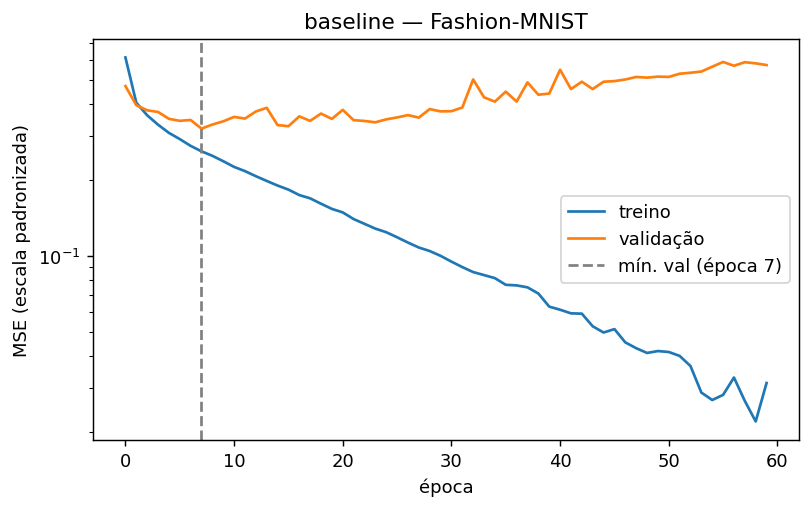
\includegraphics[width=\linewidth]{curva_mnist_baseline.png}
\caption{Baseline.}
\end{subfigure}
\hfill
\begin{subfigure}{0.48\textwidth}
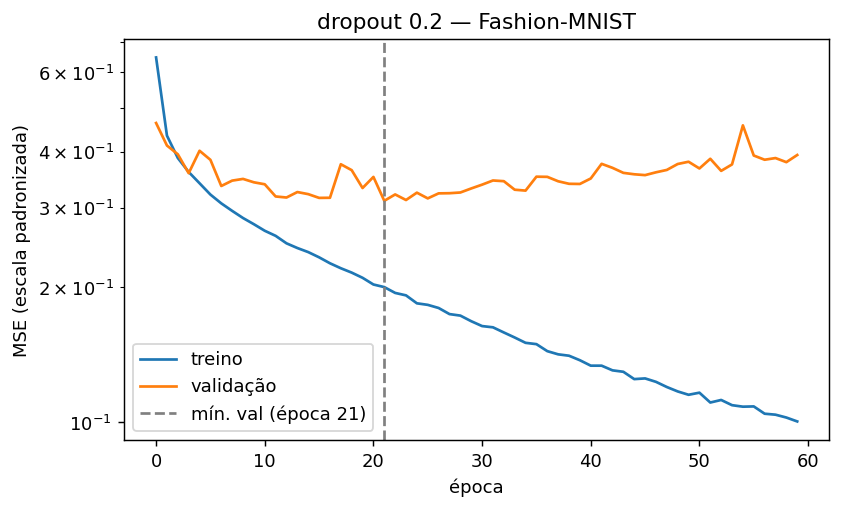
\includegraphics[width=\linewidth]{curva_mnist_dropout_02.png}
\caption{Com \emph{dropout} $0{,}2$.}
\end{subfigure}
\caption{Evolução do treino e da validação no Fashion-MNIST, escala logarítmica.}
\label{fig:clf-curvas}
\end{figure}

\begin{figure}[htbp]
\centering
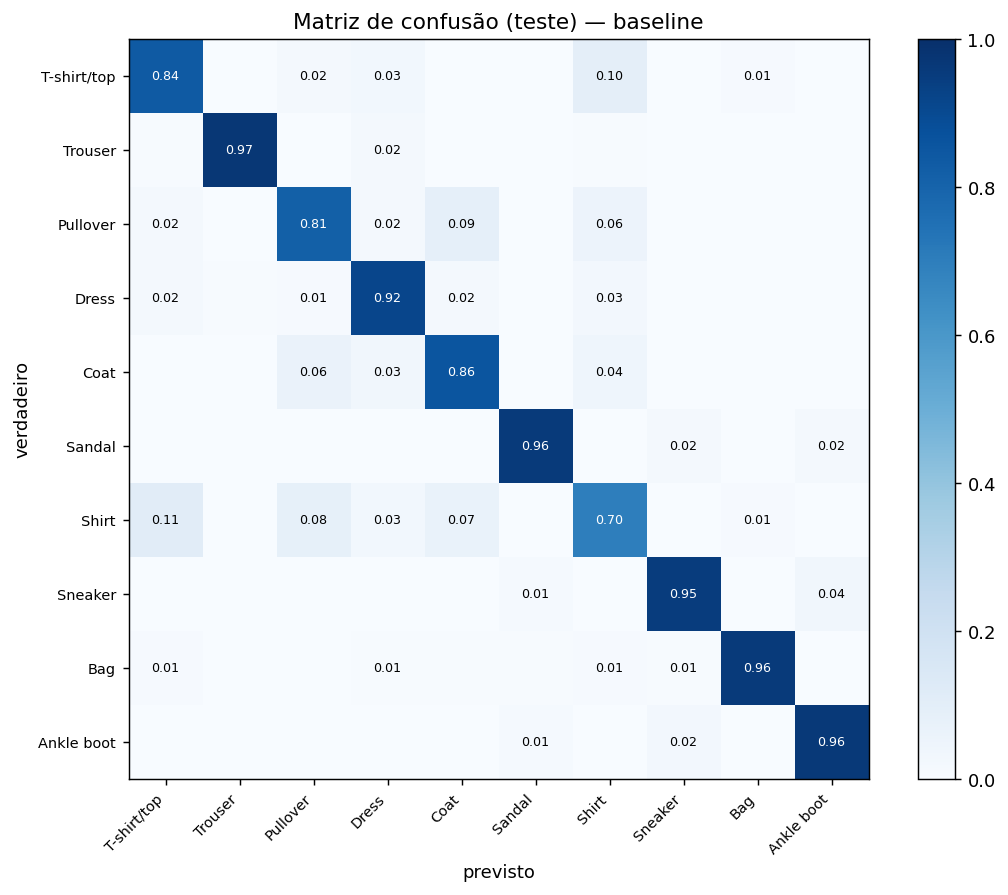
\includegraphics[width=0.72\textwidth]{confusao_baseline.png}
\caption{Matriz de confusão do baseline no conjunto de teste, normalizada por linha.}
\label{fig:confusao}
\end{figure}

As três classes de menor revocação são \emph{Shirt} ($0{,}698$), \emph{Pullover}
($0{,}815$) e \emph{T-shirt/top} ($0{,}839$); as demais superam $0{,}92$, com
\emph{Trouser} em $0{,}97$ e os três tipos de calçado acima de $0{,}95$.

Os erros não se distribuem aleatoriamente, mas concentram-se em um bloco semanticamente
coerente. \emph{Shirt} é confundida com \emph{T-shirt/top} ($0{,}11$), \emph{Pullover}
($0{,}08$) e \emph{Coat} ($0{,}07$); reciprocamente, \emph{T-shirt/top} é atribuída a
\emph{Shirt} em $0{,}10$ dos casos, e \emph{Pullover} a \emph{Coat} em $0{,}09$. Todas as
classes problemáticas correspondem a peças de tronco superior.

A interpretação conecta-se diretamente à perda da estrutura espacial: camiseta, camisa,
pulôver e casaco possuem silhuetas praticamente idênticas, distinguindo-se por detalhes
\emph{locais} --- gola, botões, punho, textura. Como a conversão para vetor de 784
elementos eliminou a noção de adjacência entre pixels, a MLP não dispõe de mecanismo
para representar tais estruturas. \textbf{O limite de aproximadamente 89\% de acurácia
não decorre de sobreajuste, mas de representação}, o que explica por que nenhum
regularizador o desloca de forma relevante. Uma arquitetura convolucional, que opera
sobre vizinhanças, atacaria precisamente este bloco de erros.

\section{Discussão}
\label{sec:discussao}

O resultado central deste trabalho emerge da comparação entre as
Tabelas~\ref{tab:reg-abl} e~\ref{tab:clf-abl}. Os mesmos quatro componentes, implementados
no mesmo código, avaliados sob o mesmo protocolo e com as mesmas sementes, produziram
conclusões opostas:

\begin{itemize}
\item na regressão, os três regularizadores degradaram o desempenho monotonicamente, com
ótimo em zero --- doze medições, todas negativas exceto o momentum $0{,}5$;
\item na classificação, os três apresentaram melhor valor positivo, com o \emph{dropout}
positivo em todos os valores testados.
\end{itemize}

A explicação é a quantidade de sobreajuste disponível. Na regressão, a razão entre erros
de treino e validação era de $1{,}9\times$, sem degradação temporal, e o $R^2$ distava
$0{,}011$ do teto imposto pelo ruído: não havia variância excessiva a ser removida, e a
penalização apenas introduziu viés. Na classificação, a razão era de $18{,}2\times$, com
pico da validação na época 7 de 60: havia ampla variância a recuperar.

Dois pontos merecem qualificação. Primeiro, \textbf{nenhum ganho individual na
classificação supera dois erros-padrão} --- o melhor deles, \emph{dropout} $0{,}2$, atinge
$1{,}87$ no teste. Afirmar superioridade com base em uma medição isolada excederia o que
três sementes sustentam. O que se sustenta é a mudança do \emph{padrão}: três resultados
positivos em três no \emph{dropout}, contra doze negativos na regressão, além do efeito
inequívoco nas métricas de sobreajuste.

Segundo, os dois problemas apresentam limites de natureza distinta. Na regressão, o
limite é o ruído ($R^2_{\max} = 0{,}987$, contra $0{,}976$ obtidos) somado à
impossibilidade de representar a descontinuidade. Na classificação, o limite é a
ausência de estrutura espacial na entrada, evidenciada pelo bloco de confusão entre peças
de vestuário superior. Em nenhum dos casos o fator limitante é aquele que os componentes
avaliados se propõem a corrigir --- o que explica a modéstia dos ganhos observados.

\section{Conclusão}

Construíram-se dois modelos MLP de referência por busca coordenada
(\texttt{[128,128]} com lr $0{,}05$ para regressão; \texttt{[256,256]} com lr $0{,}1$ para
classificação) e avaliaram-se quatro componentes adicionados isoladamente, com três
sementes por configuração.

Os resultados finais em teste são $R^2 = 0{,}9829 \pm 0{,}0018$ para a regressão e
acurácia de $0{,}8895 \pm 0{,}0044$ para a classificação, com o \emph{dropout} $0{,}2$
alcançando $0{,}8948 \pm 0{,}0022$ nesta última. Nenhum componente produziu ganho
estatisticamente demonstrável em acurácia ou $R^2$; o \emph{dropout}, contudo, exibiu
efeito grande e inequívoco sobre as métricas de sobreajuste na classificação.

Três achados metodológicos merecem destaque. A comparação de arquiteturas sob orçamento
de épocas insuficiente inverteu o ranking observado, o que justifica calibrar o orçamento
previamente. A métrica adotada para decisão determinou o que foi possível observar,
ocultando quase integralmente o efeito do \emph{dropout} quando se considerou apenas a
acurácia. E o emprego de três sementes revelou-se indispensável, não por reduzir ruído,
mas por fornecer o critério que distingue ganho de variação --- critério que, aplicado
consistentemente, rejeitou a rede maior em um problema e a aceitou no outro.

\begin{thebibliography}{9}
\bibitem{rumelhart}
RUMELHART, D. E.; HINTON, G. E.; WILLIAMS, R. J.
\emph{Learning representations by back-propagating errors}.
Nature, v. 323, p. 533--536, 1986.

\bibitem{srivastava}
SRIVASTAVA, N. et al.
\emph{Dropout: A Simple Way to Prevent Neural Networks from Overfitting}.
Journal of Machine Learning Research, v. 15, p. 1929--1958, 2014.

\bibitem{fashion}
XIAO, H.; RASUL, K.; VOLLGRAF, R.
\emph{Fashion-MNIST: a Novel Image Dataset for Benchmarking Machine Learning Algorithms}.
arXiv:1708.07747, 2017.
\end{thebibliography}

\end{document}
